\documentclass[prl,twocolumn,superscriptaddress,showpacs,floatfix]{revtex4}
\usepackage{graphicx,amsmath,amssymb,bm}
\usepackage{amsfonts}

\begin{document}

\title{Quantality and correlation measures in many-body systems}
\author{A.~Ekstr\"om}
\affiliation{Department of Physics, University of Oslo, N-0316 Oslo, Norway}
\affiliation{Department of Fundamental Physics, Chalmers University of Technology, SE-412 96 G{\"o}teborg, Sweden}
\author{G.~Hagen}
\affiliation{Physics Division, Oak Ridge National Laboratory,
Oak Ridge, TN 37831, USA}
\affiliation{Department of Physics and Astronomy, University of
Tennessee, Knoxville, TN 37996, USA}
\author{M.~Hjorth-Jensen}
\affiliation{Department of Physics, University of Oslo, N-0316 Oslo, Norway}
\affiliation{National Superconducting Cyclotron Laboratory and Department of Physics and Astronomy, Michigan
  State University, East Lansing, MI 48824-1321, USA}
\author{J.~H\o gberget}
\affiliation{Department of Physics, University of Oslo, N-0316 Oslo, Norway}
\author{G.~R.~Jansen}
\affiliation{Department of Physics and Astronomy, University of
Tennessee, Knoxville, TN 37996, USA}
\affiliation{Physics Division, Oak Ridge National Laboratory,
Oak Ridge, TN 37831, USA}
\author{A.~O.~Macchiavelli}
\affiliation{Lawrence Berkeley National Laboratory,  Nuclear Science Division, Berkeley, CA 94720-8153, USA}
 

\begin{abstract}
\end{abstract}

\pacs{21.10.-k, 21.10.Dr, 21.10.Hw, 21.10.Tg, 21.30.-x, 21.60.De, 27.30.+t}

\maketitle 

The "quantality" parameter $\Lambda = h^2/(Ma^2V_0)$,
introduced by de Boer and others in studies of gas solids
\cite{mottelson1999}, measures, in a loose sense, the strength of a
two-body (or more complicated many-body force), $V_0$, expressed in
units of the quantal kinetic energy associated with a localization of
a constituent particle of mass $M$ within the distance $a$
corresponding to the radius of the force at maximum attraction. For
small $\Lambda$ the quantal effect is small and the ground state of
the many body system will be, as in classical mechanics, a
configuration in which each particle finds a static optimal position
with respect to its nearest neighbors. If $\Lambda$ is big enough the
ground state may be a quantum liquid in which the individual particles
are delocalized and the low-energy excitations (quasi-particles) have
infinite mean free path.  A parameter related to $\Lambda$ was first
used by de Boer in the analysis of quantal constants of the noble gas
solids.

The aim of this work is to study in more detail the above quantality
parameter by using the expectation values of the kinetic and potential
energies obtained from {\em ab initio} calculations of various quantum
mechanical systems. In particular we focus on quantum dots and
nuclei. The aim is extract information about correlations in
complicated many-particle systems. Quantum dots have been chosen as
one of the systems due to the possibility to tune the frequency of the
trapping potential. With a small frequency we enter a region where
correlations induced in the potential energy become more important
with respect to the kinetic energy, leading thus to a decrease in
$\Lambda$. Similarly, for nuclei, we investigate the role of two-body
and three-force in chains of isotopes like the oxygen, calcium and
nickel isotopes. The latter gives us the possibility to study the
evolution of $\Lambda$ as a function of an increasing number of
neutrons.  As the system becomes more and more neutron reach, one
reaches the so-called neutron drip line, where adding one additional
neutron renders the nucleus unstable with respect to one-neutron decays. 
Towards the drip line, nuclei become weakly bound, reflected in a diminishing
separation energy (give definition). This is reflected in a dimishing value of the kinetic and potential energies. 
\begin{figure}%[hbtp]
     \begin{center}
            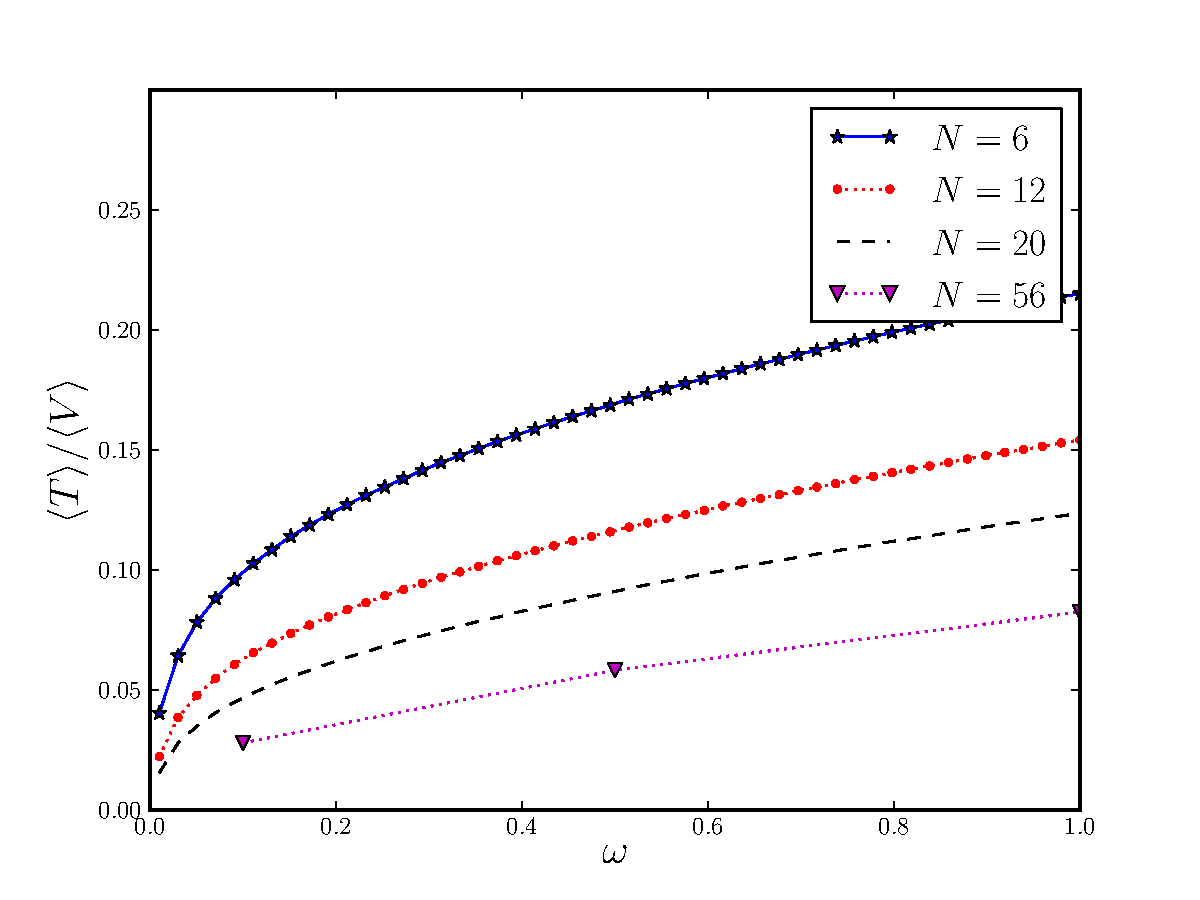
\includegraphics[width=0.38\textwidth]{figures/qdots.pdf}
    \end{center}
    \caption{Diffusion Monte Carlo results for the ratio $\langle T \rangle/\langle V\rangle$ as function of 
the oscillator frequency $\omega$.}
   \label{fig:qdots}
\end{figure}


\begin{acknowledgments}
  This work was supported by the Office of Nuclear Physics,
  U.S.~Department of Energy (Oak Ridge National Laboratory). This research used computational resources of the
  National Center for Computational Sciences, the National Institute
  for Computational Sciences, the Notur project in Norway and the Research Council of Norway under project ISP-Fysikk/216699. 
\end{acknowledgments}




\begin{thebibliography}{99}

\bibitem{mottelson1999} B.~R.~Mottelson, Nucl.~Phys.~A {\bf 649}, 45 (1999).


\end{thebibliography}


\end{document}






